
\chapter{Project Management}
\label{cha:management}

The week-to-week management of your project is documented in your weekly
progress reports, so you do not need to repeat that information here. A number
of important points that you need to address are:
\begin{itemize}
\item What are the main components of the project (or \emph{workpackages}) that have to be completed for it to succeed?
\item What software process model (e.g. waterfall or evolutionary)
did you use for \emph{individual workpackages}?
\item How did you allocate team members to particular tasks?
\item How did you coordinate what team members were working on?
\item How did you communicate the relevant technical information in the
team?
\end{itemize}
Note that a clean design makes all of these easier, so you could
refer to your design section, i.e. chapter~\ref{cha:design}, where
appropriate. You can also discuss difficulties in the team
interactions if there were any, and how you dealt with them.

\begin{figure}
  \centering
  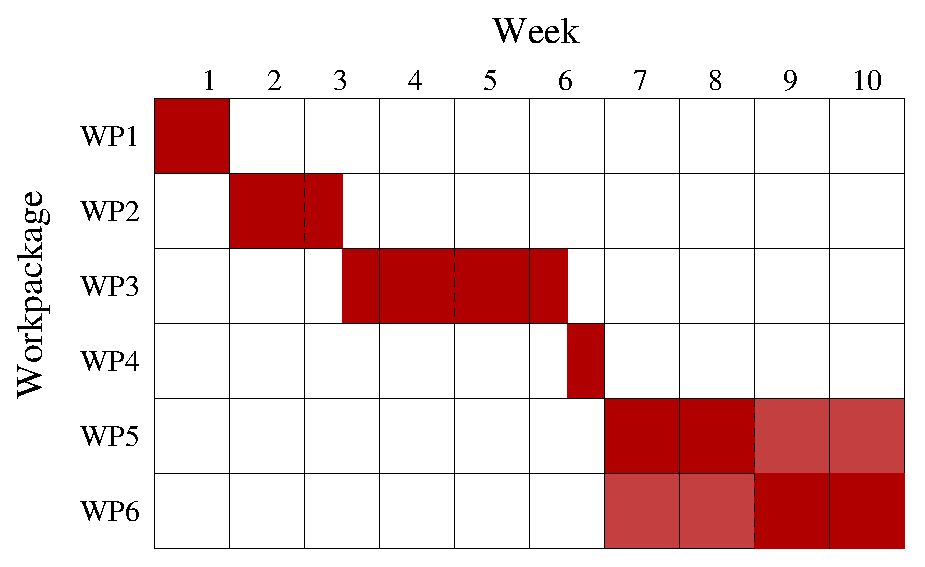
\includegraphics[width=.5\textwidth]{gant}
  \caption{Example timeplan of a project.}
  \label{fig:timeplan}
\end{figure}
You can, for example, include a chart detailing the time management of your
project as shown in figure~\ref{fig:timeplan}. Explain the single workpackages
in the text:
\begin{description}
\item[Workpackage 1:] Requirements specification
  \hfill (Week 1)
\item[Workpackage 2:] Something else\ldots
  \hspace*{\fill} (Week 2---3)
\item[Workpackage 3:] \ldots
\end{description}
This is only an example chart, of course; your own timeplan will
probably look differently. Note that different workpackages can be
worked on in parallel!

Figures are included in {\LaTeX} as \texttt{.eps} files. In Linux
you can use \texttt{convert} to convert any type of graphics file to
\texttt{.eps} format.
